% Anhang A
\section{Fertigungszeichnungen}
\label{anh:fertigungszeichnungen}
Der Anhang ist gut geeignet um \glqq{}der Vollständigkeit halber\grqq{} Informationen zur Verfügung zu stellen, die aber für das eigentliche Verständnis des im Dokument vermittelten ingenieurwissenschaftlichen Verständnis nicht notwendig oder dafür unwesentlich sind. 

Ein gutes Beispiel für derartige Informationen sind häufig Detailinformationen, die für das Konzept nicht wesentlich sind, wie Fertigungszeichnungen. 
Häufig ist die ingenieurwissenschaftliche Aufgabe die Erstellung eines Konzepts, ein Konstruktion und die anschließende Überprüfung des Konzepts mit Hilfe einer prototypischen Implementierung. 
Wie genau die Fertigungszeichnungen aussehen und welche Toleranzen dabei genau einzuhalten sind, ist oft für das Verständnis nicht entscheidend. 
Daher können derartige Informationen dann gut in den Anhang landen. 

Vorsicht: Diese Aussagen gelten natürlich nicht, wenn beispielsweise die Wirkung von bestimmten Passungen und Toleranzabhängigkeiten im rahmen der Arbeit zu untersuchen sind. 
Dann spielen genau diese Angaben natürlich eine wichtige Rolle; in dem Fall ist zu überdenken, ob diese Informationen und Fertigungszeichnungen nicht doch in den Hauptteil der Arbeit gehören. 



% Anhang B
\section{Layouts}
\label{anh:layouts}
Die Aussage für die Details der Konstruktion in den Fertigungszeichnungen in Anhang~\ref{anh:fertigungszeichnungen} ist sinngemäß auf elektrische / elektronische Layouts und Platinendetails zu übertragen. 


% Anhang C
\section{Datenblätter und Zeichnungen}
\label{anh:datenblaetter}
%
Häufig ist bei Aufgaben, die eine Erstellung eines Konzeptes oder Konstruktion beinhalten auf Datenblätter von Bauteilen bzw.~Komponenten zu verweisen. 
Um den Leser der Dokumentation nicht zu, Suchen und Herunterladen der Datenblätter zu zwingen, ist es höflich und sinnvoll, auf die für die Arbeit relevanten Passagen oder Teile des Datenblatts im Anhang zu verweisen. 
Diese Auszüge aus Datenblättern gehören dann üblicherweise hier in den Anhang.


\begin{figure}[H]
  \begin{center}
    
\includegraphics[width=0.5\textwidth]{bilder/bologo}
      % Einbinden einer Pixelgrafik.
      % Die Endung „.png“ darf weggelassen werden.
\end{center}
\caption{Das Bo-Logo der Hochschule Bochum mit CVH-Zusatz für den Campus Velbert/Heiligenhaus}
\label{fig:AnhC_Bild1}
\end{figure}

In dem Zusammenhang kommt es vor, dass Sie gerne ein Bild oder eine Tabelle anfertigen möchten, die Passagen oder Details aus dem Datenblatt enthalten  (siehe Bild~\ref{fig:AnhC_Bild1}) oder Tabelle (vgl.~\ref{tab:AnhC_tabelle1}). 



\begin{table}[H]
\caption{Unterschiedliche Logos mit Text der Hochschule Bochum im Verzeichnis \glqq{}bilder\grqq{}}
\label{tab:AnhC_tabelle1}
\begin{center}
\begin{tabular}{||c|c||}
\hline\hline
logo-hochschule-bochum-cvh-text.pdf & logo-hochschule-bochum-text.pdf\\ \hline

\includegraphics[width=4cm]{bilder/logo-hochschule-bochum-cvh-text.pdf} & 

\includegraphics[width=4cm]{bilder/logo-hochschule-bochum-text.pdf} \\
\hline\hline
\end{tabular}
\end{center}
\end{table}




%%%%%%%%%%%%%%%%
\section{Weitere \LaTeX{}-Beispiele, Tikz und Einbinden von csv-Dateien und xls}
\label{sec:csv+xls}
%

Eine Gleichungsnummer im Anhang erscheint mit automatischer Nummerierung, wie im Haupttext auch. 
Die Abschnittsnummern sind jedoch nicht mehr arabische sondern mit Hilfe von Buchstaben nummeriert, wie das folgende Beispiel zum Satz des Pythagoras zeigt: 
%
\begin{equation}
\label{eq:AnhC_SatzPythagoras}
C^2 = A^2+B^2
\end{equation}
%
Das gleiche gilt auch für ein Bild (siehe Bild~\ref{fig:AnhC_Bild2}) oder eine Tabelle (vgl.~\ref{tab:AnhC_tabelle2}). 


\begin{table}[H]
\caption{Testtabellenüberschrift}
\label{tab:AnhC_tabelle2}
\begin{center}
\begin{tabular}{||r|c|c|c|c|c|c||}
\hline \hline 
\# 		& 1 & 2 & 3 & 4 & 5 & 6\\ \hline
Monat 	& Januar & Februar & März & April & Mai & Juni \\
\hline \hline 
\end{tabular}
\end{center}
\end{table}


\begin{figure}[H]
\begin{center}
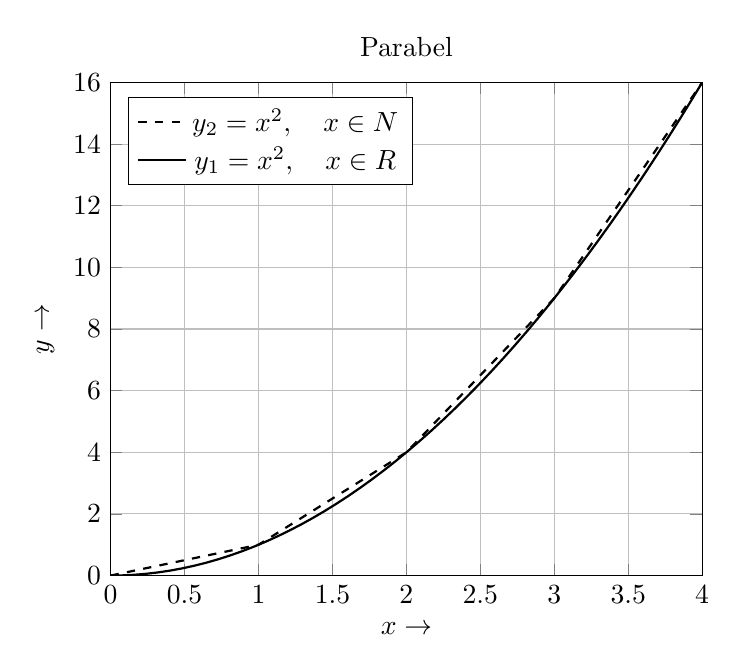
\begin{tikzpicture}
    \begin{axis}[
     width=.75\columnwidth,
     title = {Parabel}, 
     xlabel={$x \rightarrow$},
     ylabel={$y \rightarrow$},
     xmode=normal, % kann weggelassen werden
     ymode = normal, % kann weggelassen werden
     xmin=0, xmax=4,
     ymin=0, ymax=16,
%     ytick={ 90, 0, -90},
     legend pos={north west},
%     yticklabels=\empty , 
%     /pgfplots/ytick={0,-45,-90,-135,-180} , 
%    grid = minor, % alle Zehnerpotenzen und eine Nachkommastelle
    grid = major, % alle Zehnerpotenzen 
     ]
     \addplot[color=black, thick,dashed]
     coordinates{
     (0,0)
     (1,1)
     (2,4)
     (3,9)
     (4,16)
     };
     \addlegendentry{$y_2=x^2, \quad x\in\mathbb{N}$}
	% Phasengang nach Musterlösung D=0.1 w0 = 1 K=1
     \addplot[color=black, thick,solid, samples=200, 	domain=0:16    ]
     { 0 + \x^2   };
     \addlegendentry{$y_1=x^2, \quad x\in\mathbb{R}$}
     \end{axis}
\end{tikzpicture}
\end{center}
\caption{Testbildunterschrift für eine mit tikz dargestellte Funktion}
\label{fig:AnhC_Bild1-einfach}
\end{figure}

\begin{figure}[H]
\begin{center}
%$A^2 + B^2 = C^2$


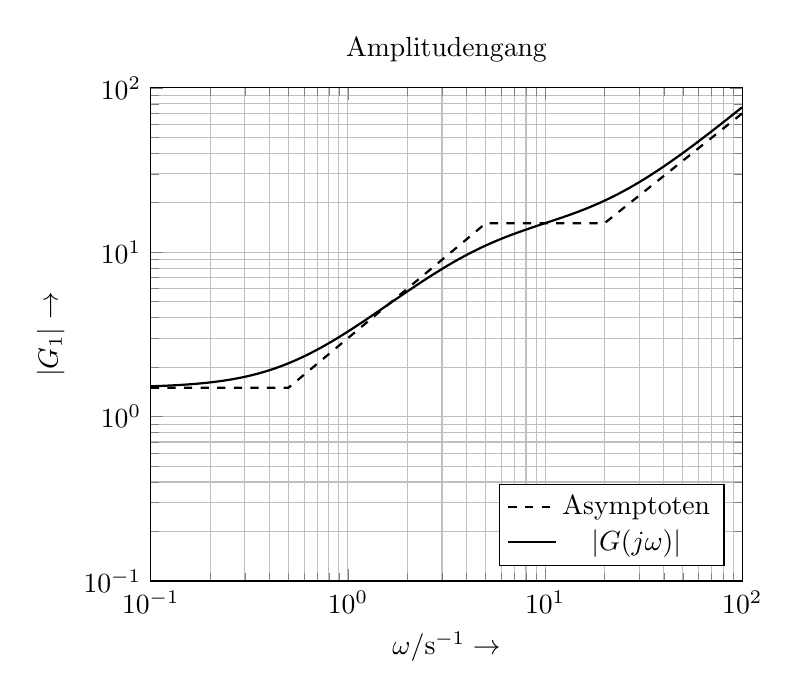
\begin{tikzpicture}
    \begin{loglogaxis}[
     width=.75\columnwidth,
     title = {Amplitudengang}, 
     xlabel={$\omega$/s$^{-1} \rightarrow$},
     ylabel={$|G_1| \rightarrow$},
     xmin=10^(-1), xmax=10^(+2),
     ymin=10^(-1), ymax=10^(+2),
     max space between ticks=11,
     legend pos={south east},
     grid = minor % alle Zehnerpotenzen und eine Nachkommastelle
%     grid = major % alle Zehnerpotenzen 
     ]
     \addplot[color=black, thick,dashed]
     coordinates{
     (1e-1,  	1.5e0)
     (5e-1,  	1.5e0)
     (5e0,  	1.5e1)
     (2e+1,  	1.5e1)
     (1e+2,  	7e+1)
     };
     \addlegendentry{Asymptoten}
     \addplot[color=black, thick,solid, samples=200, 	domain=10^(-1):10^(2)]
     {
     1.5 * 								% P  
     (1 + (1/5e-1)^2*\x^2)^0.5 *	% PD
     1/(1 + (1/5e0)^2*\x^2)^0.5 *	% PT1
     (1 + (1/2e+1)^2*\x^2)^0.5 *	% PD
     1									% Ende
     };
%	{0.2*1.0*(1+(1/4.0e-1)^2*\x^2)^0.5 * 1.0/((1-(1/1.0)^2*\x^2)^2+(2*0.1*1/1.0*\x)^2)^0.5*1.0/(1+(1/10)^2*\x^2)^0.5/(1+(1/10)^2*\x^2)^0.5}; % Amplitudengang nach Musterlösung D=0.1 w0 = 1 K=1
     \addlegendentry{$|G(\text{j}\omega)|$}
     \end{loglogaxis}
% %%%% weitere Zeichnungen außerhalb der Logarithmischen Skala: 
%     \draw[thick, dashed] (4.0e-1, 1.141) -- (1e0, 1.141)  node[right] {3dB};
%     \draw[thick, dashed] (0.4, 1.0) -- (1.0, 1.0) ;
\end{tikzpicture}

\begin{tikzpicture}
    \begin{axis}[
     width=.75\columnwidth,
     title = {Phasengang}, 
     xlabel={$\omega$/s$^{-1} \rightarrow$},
     ylabel={$\varphi_1 (\text{j}\omega) \rightarrow$},
     xmode=log,
     ymode = normal,
     xmin=10^(-1), xmax=10^(2),
     ymin=-95, ymax=95,
     max space between ticks=90
     try min ticks=180,
     ytick={ 90, 0, -90},
     legend pos={south west},
%     yticklabels=\empty , 
%     /pgfplots/ytick={0,-45,-90,-135,-180} , 
%    grid = minor, % alle Zehnerpotenzen und eine Nachkommastelle
    grid = major, % alle Zehnerpotenzen 
     ]
     \addplot[color=black, thick,dashed]
     coordinates{
     (1e-1,   	0)
     (5.0e-1),  0)
     (5.0e-1,  90)
     (5.0e0,  90)
     (5.0e0,  0)
     (2.0e+1,  0)
     (2.0e+1,  90)
     (1.0e+2,  90)
     };
     \addlegendentry{Asymptoten}
	% Phasengang nach Musterlösung D=0.1 w0 = 1 K=1
     \addplot[color=black, thick,solid, samples=200, 	domain=10^(-1):10^(2)    ]
     { 0 
     %####Achtung#### atan2 ist nicht in allen pgfplot-Versionen enthalten!
     %+ atan2(((1/5e-1)*\x),1)  		% PD
     %+ atan2(( -(1/5e0)*\x) , 1 )		% 2* PT1
     %+ atan2(((1/2e1)*\x),1)  		% PD
     };
     \addlegendentry{$\varphi (\text{j}\omega)$}
     \addplot[color=blue, thick,solid, samples=200, 	domain=10^(-1):10^(2)    ]
     { 
     0  		% P
     };     
    	\draw (3.5, 1000) node[blue] {$\varphi_\text{i}$} ; 
     \addplot[color=blue, thick,solid, samples=200, 	domain=10^(-1):10^(2)    ]
     { 
     %+ atan2((1/5e-1)*\x,1)  		% PD
     0
     };     
    	\draw (0.3, 1750) node[blue] {$\varphi_\text{ii}$} ; 
     \addplot[color=blue, thick,solid, samples=200, 	domain=10^(-1):10^(2)    ]
     { 
     %+ atan2( -(1/5e0)*\x , 1 )		% 2* PT1
     0
     };
    	\draw (1.1, 500) node[blue] {$\varphi_\text{iii}$} ; 
     \addplot[color=blue, thick,solid, samples=200, 	domain=10^(-1):10^(2)    ]
     {
     0
     %+ atan2((1/2e1)*\x,1)  		% PD
     };
    	\draw (0.3, 1050) node[blue] {$\varphi_\text{iv}$} ; 
     \end{axis}
\end{tikzpicture}


\end{center}
\caption{Testbildunterschrift für ein mit tikz erstelltes Bode-Diagramm}
\label{fig:AnhC_Bild2}
\end{figure}




%
Das Einbinden von csv-Dateien (Messungen ) kann entweder über ein Bild (Bitmap) erfolgen oder aber auch unter  \LaTeX{}.
Notwendig ist dafür das Laden des Pakets \newline 
\texttt{$\backslash$usepackage{pgfplots}}. 

\begin{figure}
    \centering
    \begin{tikzpicture}
        \begin{axis}[
            title=Datenimport mit tikz,
            xlabel={$x$},
            ylabel={$y$},
            ]
            \addplot[blue] table [x=A1, y=A2, col sep=tab] {daten/data.txt};
            \addplot[red] table [x=A1, y=A3, col sep=semicolon] {daten/data.dat};
            \addplot[green] table [x=A1, y=A4, col sep=comma] {daten/data.csv};
        \end{axis}
    \end{tikzpicture}
	\caption{Darstellung von Messdaten aus verschiedenen Formaten: txt, dat und csv}
	\label{fig:Beispielmessung-csv}
\end{figure}  






